%%%%%%%%%%%%%%%%%%%%%%% file template.tex %%%%%%%%%%%%%%%%%%%%%%%%%
%
% This is a template file for Web of Conferences Journal
%
% Copy it to a new file with a new name and use it as the basis
% for your article
%
%%%%%%%%%%%%%%%%%%%%%%%%%% EDP Science %%%%%%%%%%%%%%%%%%%%%%%%%%%%

\documentclass{webofc}
% option "twocolumn" for typesetting an article in two columns format (default one column)
% \documentclass[twocolumn]{webofc}

\usepackage[varg]{txfonts}   % Web of Conferences font
\usepackage{hyperref}
\usepackage{url}
%%%%%%%%%%%%%%%%%%%%%%%%%%%%%%%%%%%%%%%%%%%%%%%%%%%%%%%%%%%%%%%%%%%%%%%%%%%%%
\hypersetup{colorlinks=true,citecolor=blue,urlcolor=blue,linkcolor=blue}
%%%%%%%%%%%%%%%%%%%%%%%%%%%%%%%%%%%%%%%%%%%%%%%%%%%%%%%%%%%%%%%%%%%%%%%%%%%%%
%
% Put here some packages required or/and some personnal commands
%
%
\begin{document}
%
\title{Exploiting Kubernetes to Simplify the Deployment and Management of the Multi-purpose CMS Pilot Job Factory}
%
% subtitle is optionnal
%
%%%\subtitle{Do you have a subtitle?\\ If so, write it here}


\author{
\firstname{Jeffrey Michael} \lastname{Dost} \inst{1}\fnsep\thanks{\email{jdost@ucsd.edu}}
\and
\firstname{Marco} \lastname{Mascheroni} \inst{1}\fnsep\thanks{\email{marco.mascheroni@cern.ch}}
\and
\firstname{Brian Paul} \lastname{Bockelman} \inst{2}
\and
\firstname{Colby} \lastname{Walsworth} \inst{1}
\and
\firstname{Edita} \lastname{Kizinevic} \inst{3}
\and
\firstname{John} \lastname{Thiltges} \inst{4}
\and
\firstname{Merina} \lastname{Albert} \inst{5}
\and
\firstname{Vaiva} \lastname{Zokaite} \inst{6}
\and
\firstname{Frank} \lastname{Würthwein} \inst{1}on behalf of the CMS collaboration
}

\institute{
University of California San Diego
\and
Morgridge Institute for Research
\and
CERN
\and
University of Nebraska--Lincoln
\and
Fermi National Accelerator Lab
\and
Vilnius University
}

\abstract{
GlideinWMS, a widely utilized workload management system in high-energy physics (HEP) research, serves as the backbone for efficient job provisioning across distributed computing resources. It is utilized by various experiments and organizations, including CMS, OSG, Dune, and FIFE, to create HTCondor pools as large as 600k cores. In particular, a shared factory service historically deployed at UCSD has been configured to interface with more than 500 routes to compute clusters. As part of our team's initiative to modernize infrastructure and enhance scalability, we undertook the migration of the GlideinWMS factory service into the Kubernetes environment. Leveraging the flexibility and orchestration capabilities of Kubernetes, we successfully deployed the factory service within the OSG Tiger Kubernetes cluster. The major benefits Kubernetes gives us is it streamlines the management and monitoring of the factory infrastructure, and improves fault tolerance through its resilient deployment strategies. Through this case study, we aim to share insights, challenges, and best practices encountered during the migration process. Our experience underscores the benefits of embracing containerization and Kubernetes orchestration for HEP computing infrastructure, paving the way for scalability and resilience in distributed computing environments.
}
%
\maketitle
%
\section{Introduction}
\label{intro}
GlideinWMS (Glidein Workflow Management System)\cite{gwms} is a pilot-based workload manager. It used in distributed computing, and is the core set of services that powers the submission infrastructure for the Compact Muon Solenoid (CMS) experiment at CERN\cite{cms}. GlideinWMS dynamically provisions execute points, known as glideins, across grid and cloud resources. It then fetches jobs from a central queue for efficient execution. Benefits of GlideinWMS are that it simplifies workflow management and optimizes resource usage. It also ensures scalable and flexible job execution in complex environments.

% add overview of how gwms works, components
GlideinWMS consists of two core components: the frontend and the factory, which together deploy a dynamic HTCondor pool\cite{htcondor}, as depicted in Figure \ref{GWMSExplanation}. The GlideinWMS frontend continuously monitors job queues at the HTCondor access points. When jobs are detected, the frontend evaluates resource requirements and sends requests to a GlideinWMS factory. The factory, in turn, provisions pilot jobs, the glideins, by submitting them to compute elements (CEs) on the Worldwide LHC Computing Grid (WLCG)\cite{wlcg} and OSG affiliated institutions. These pilot jobs initialize execution points by setting up an HTCondor worker node environment on the allocated resources. Once active, the glideins autonomously connect back to the HTCondor central manager, pulling real user jobs from the central queue for execution. This architecture effectively abstracts the complexities of the underlying infrastructure, transforming a heterogeneous set of computing resources into a unified, dynamically scalable environment. By leveraging this mechanism, CMS and other virtual organizations (VOs) can utilize available computing power without the need for direct job submission to individual resource providers (sites) and create heterogeneous and dynamic HTCondor pools with more than 500k cores\cite{globalpool}.

\begin{figure}[h]
\centering
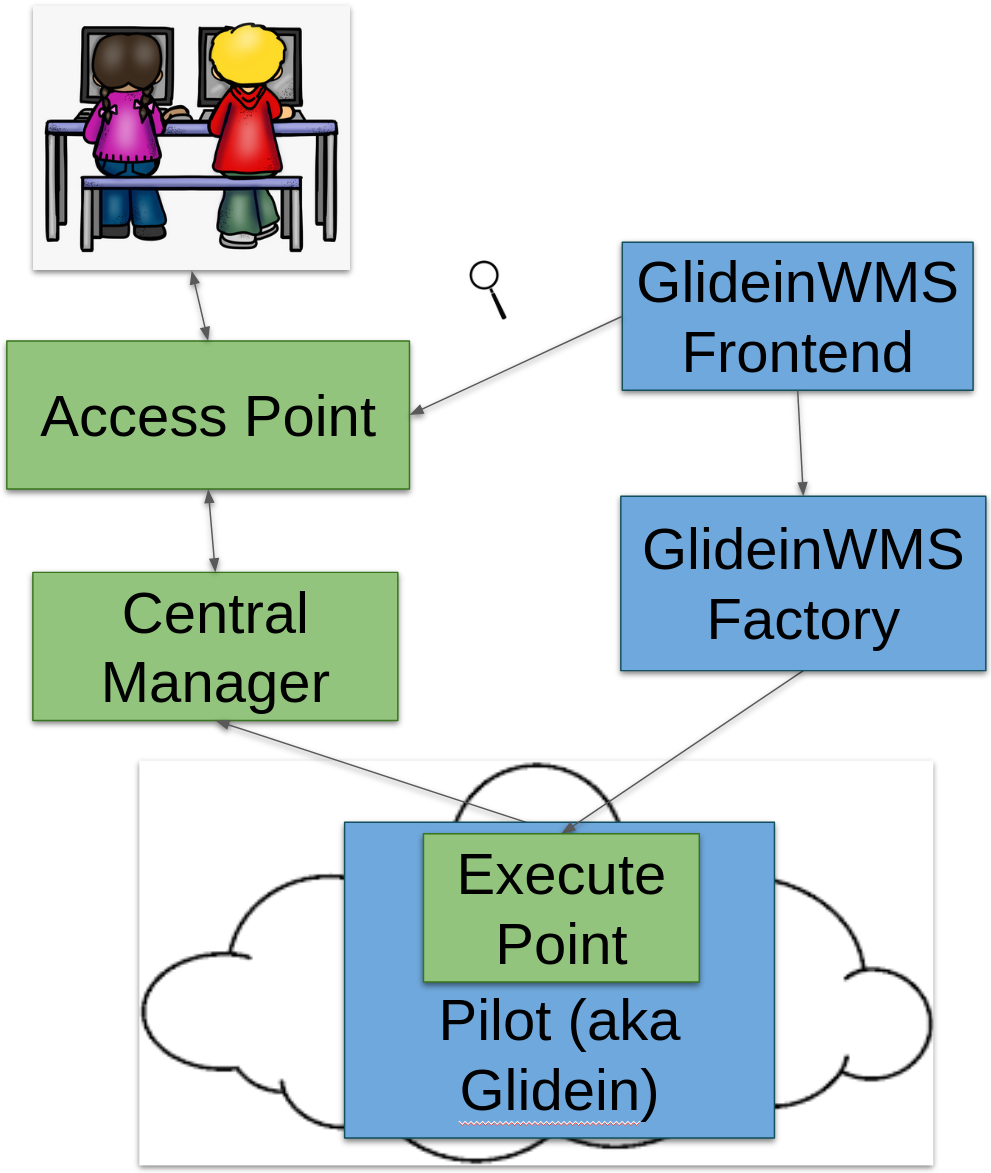
\includegraphics[width=6cm,clip]{images/GWMSExplanation}
\caption{Main Components of a GlideinWMS deployment}
\label{GWMSExplanation}
\end{figure}

The Factory Operations team is a collaboration between CMS and OSG. It manages multiple factories that provide access to different subsets of compute sites. The factories serve distinct GlideinWMS frontends, which support various VOs using the system. The Fermi National Accelerator Laboratory (FNAL) Factory serves CMS at  US Tier-2 (T2) and Tier-1 (T1) sites, while the CERN Factory handles glidein submission for all CMS sites globally. The OSG Factory provides a more general purpose service, supporting a broader range of VOs.  In addition to CMS, scientific collaborations such as IceCube, LIGO, DUNE, and GlueX operate a GlideinWMS frontend and use the OSG Factory to create dynamic HTCondor pools and access distributed computing resources. On the OSG side alone, about a dozen scientific experiments and nearly 100 individual research groups leverage a single GlideinWMS frontend\cite{osgprojects}. This setup ensures resource distribution tailored to the needs of each organization, enhancing scalability and redundancy. The topology of the most active GlideinWMS factories and frontends deployed around the world is shown in Figure \ref{GWMSDeployment}.

\begin{figure}[h]
\centering
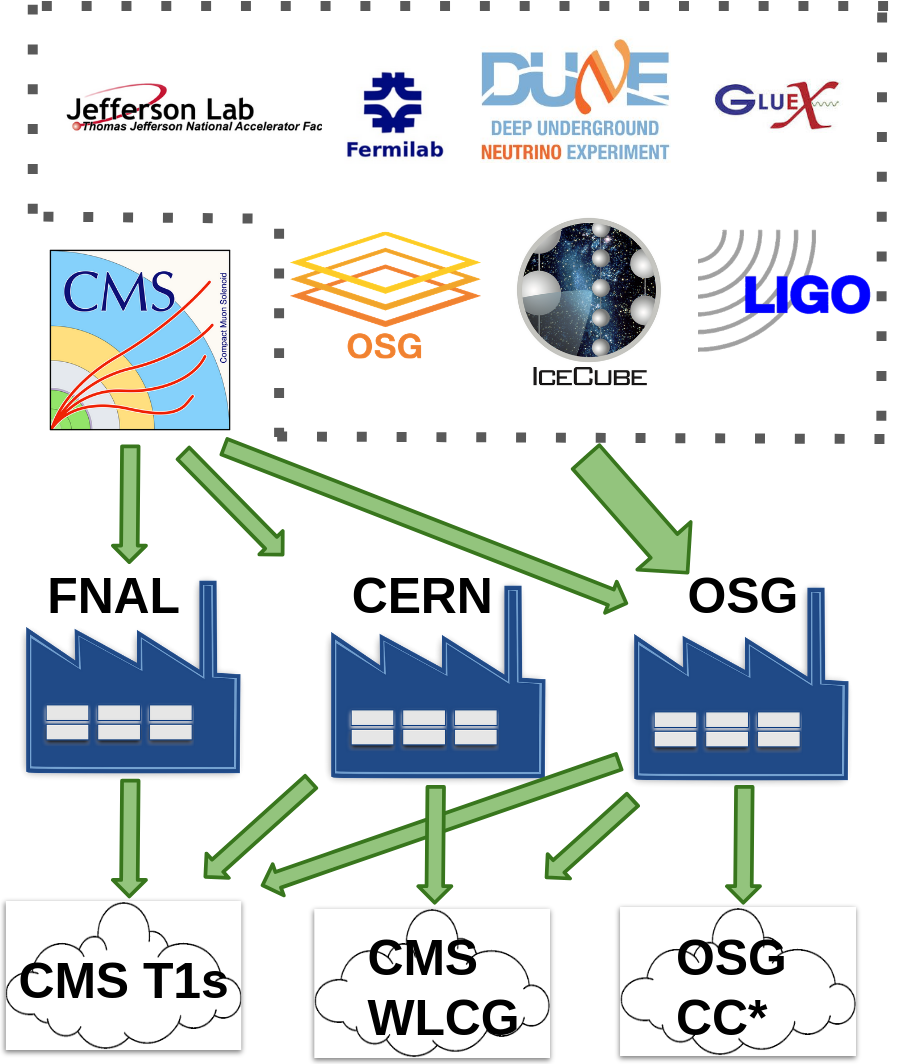
\includegraphics[width=6cm,clip]{images/GWMSDeployment}
\caption{Deployed GlideinWMS factories and frontends}
\label{GWMSDeployment}
\end{figure}

Kubernetes (K8s)\cite{k8s} is a container orchestration system that is becoming an increasingly popular tool for deploying and managing distributed compute resources. The benefits of managing services under K8s are that it brings high availability and resilience through the automation of scaling, load balancing, and failover processes. The OSG Factory has been chosen to be migrated to K8s as a part of a larger, more general push in OSG to migrate all central services under provisioning in K8s\cite{OSGfabric}. OSG services such as the GRACC accounting system, glidein pool frontends and central managers, hosted compute entrypoints (CEs), software repositories, and web pages have also undergone similar migrations. Thus, the provisioning the OSG Factory with K8s better integrates factory operations within the broader management and maintenance of OSG infrastructure.


\section{Required changes for containerization}
\label{containerization}


The first step in migrating the OSG Factory to K8s is to design a container image. OSG uses Docker\cite{docker} as its container runtime, and OSG Software provides a base Docker image that we leveraged as our starting point. This base image is built on AlmaLinux 9 and includes the OSG Yum repositories pre-configured. Additionally, it sets up supervisord to manage services and provides startup script hooks that allow arbitrary scripts to be executed at runtime before launching services. These hooks provide the flexibility needed to build a fully functional GlideinWMS factory container by extending the OSG Software base image.

Setting up a GlideinWMS factory on a bare metal machine is not as simple as installing a few packages with Yum. The process involves several manual configuration steps that must be completed before the factory can function properly. The standard procedure includes:

\begin{enumerate}
\item Installing packages for GlideinWMS, HTCondor, and httpd
\item Updating configuration files for HTCondor and the factory
\item Downloading required HTCondor tarballs for glideins
\item Updating factory configuration files to include downloaded tarballs
\item Cloning the factools Git repository
\item Cloning the factory entry configuration Git repository
\item Enabling various custom cron scripts
\item Running the factory upgrade command
\item Starting httpd, HTCondor, and factory services
\end{enumerate}

To fully containerize the factory, our Docker image needs to automate the entire process so that the factory would be fully operational upon container instantiation. This is achieved by writing Bash scripts to handle each step and integrating them with the startup script hooks provided by the OSG base image. While automation is a technical necessity for K8s deployment, it also brings significant operational benefits. Previously, setting up a factory from scratch required several hours of manual intervention by an operator. With the new containerized approach, the same process is now reduced to a few script executions, completing in seconds instead of hours. Beyond efficiency, this automation also ensures consistency, reproducibility, and a reduction in human error, making deployments more reliable and scalable.

\section{Required changes to factory operations procedures}
\label{procedures}

Migrating the OSG Factory to K8s introduced changes to routine procedures for the factory operations team. In bare metal factories, updating service configurations has traditionally required an operator to manually log into the host machine, modify configuration files, and restart services. While this approach is technically possible in K8s, any direct changes made inside a running container are not persistent and will be lost when the container restarts. Instead, K8s provides mechanisms to manage configuration externally using objects such as environment variables and ConfigMaps. For example, environment variables can be declared at the K8s layer to override specific settings inside a container. Additionally, the configMapGenerator object allows administrators to define configuration files that can be mounted as volumes, replacing files inside the container. These mechanisms ensure that service configurations remain persistent and can be dynamically controlled from K8s without modifying the container image itself.

To apply changes, OSG’s K8s clusters use a GitOps-based deployment model powered by Flux. Instead of directly applying K8s commands to deploy or update services, administrators modify YAML configuration files stored in a Git repository. Flux continuously monitors this repository, detects changes, and automatically updates the corresponding K8s objects, triggering container restarts if necessary. This approach ensures that all changes are version-controlled, making deployments transparent and traceable. Unlike traditional manual updates, GitOps eliminates the risk of untracked, ad-hoc modifications, ensuring that every change is logged with a clear history.

However, not all factory configurations are suitable for storage in the K8s Git repository. One such exception is the entry configuration, which defines the set of compute sites a factory can submit glideins to, along with specific resource requests (e.g., number of CPUs, memory, maximum wall-time, GPUs, etc.). Since not all GlideinWMS factories are K8s-based, these configuration files must remain externally managed to maintain compatibility with both bare metal and K8s-based factories. Previously, updating entry configurations for bare metal factories required manual steps:

\begin{enumerate}
\item Update file(s) in \verb"/etc/osg-gfactory/"
\item Run the following commands:
\begin{enumerate}
\item \verb"systemctl stop gwms-factory"
\item \verb"gwms-factory reconfig"
\item \verb"systemctl start gwms-factory"
\end{enumerate}
\end{enumerate}

To maintain GitOps consistency for K8s-based factories, we implemented a periodic cron job that runs every fifteen minutes to check for changes in the \verb"osg-factory" repository. If changes are detected, the script automatically stops, reconfigures, and restarts the factory. This approach keeps entry configurations Git-driven, aligning with the broader GitOps deployment model. Beyond ensuring consistency, this automation provides two key benefits:

    \begin{itemize}
        \item Scalability: A single Git commit can propagate changes simultaneously to multiple factories, including bare metal ones.
        \item Reduced Human Error: Unlike the manual update procedure, this automated approach eliminates the risk of missed steps or misconfigurations by operators.
    \end{itemize}

By shifting to a fully automated, GitOps-driven approach, the new workflow improves operational efficiency, reproducibility, and maintainability across OSG’s K8s-based factory infrastructure.

\section{State persistence}
\label{persistence}

In K8s, pods are ephemeral by design, meaning that the factory pod reinstalls itself from scratch every time it restarts. However, both GlideinWMS and HTCondor rely on persistent state stored on disk to function properly. To retain this state across pod restarts, K8s provides a Persistent Volume Claim (PVC) mechanism, which allows workloads to mount persistent storage volumes that remain intact even when a pod is recreated. For the OSG K8s factory, we provisioned three NVMe-backed Ceph volumes to store essential stateful data:

\begin{itemize}
\item \verb"/var/lib/condor"
\item \verb"/var/lib/gwms-factory"
\item \verb"/var/log/gwms-factory"
\end{itemize}

The choice of NVMe-backed storage was driven by the high I/O demands of the factory. Every day, O(10k) glideins are instantiated and terminated, generating significant read and write operations. Each glidein:

    \begin{itemize}
        \item Downloads hundreds of files from the factory web server upon startup.
        \item Writes logs back to the factory upon termination.
    \end{itemize}

Using SSD-based NVMe storage ensures that the factory can handle these intensive operations without I/O bottlenecks. Additionally, these Ceph-backed volumes are dynamically scalable. If additional storage is required, K8s allows us to increase volume size directly from the configuration, eliminating the need for manual interventions or pod restarts.

\section{Kubernetes resilience}
\label{resilience}

A key advantage of deploying the OSG Factory in K8s is its built-in high availability and fault tolerance. Unlike traditional bare metal deployments, where a hardware failure can cause prolonged downtime, K8s ensures that services remain operational by automatically rescheduling services to available hosts within the cluster. In a bare metal setup, if the physical machine running the factory were to fail, the factory would remain offline until an operator manually intervenes to diagnose the issue, replacing hardware if necessary, and restoring services. This process could take hours or even days, depending on the failure’s severity and the availability of replacement hardware. Additionally, recovering from a failure often requires significant manual effort, leading to longer downtime and an increased risk of human error. With K8s, this risk is mitigated. The factory pod runs inside a K8s cluster, which consists of multiple interconnected worker nodes. If the node hosting the factory pod goes down, K8s automatically detects the failure, schedules a replacement pod on another available node, and restores the factory’s state using PVCs. This ensures that no critical data is lost and that the factory resumes normal operation within minutes, requiring no manual intervention.

\begin{figure}[h]
\centering
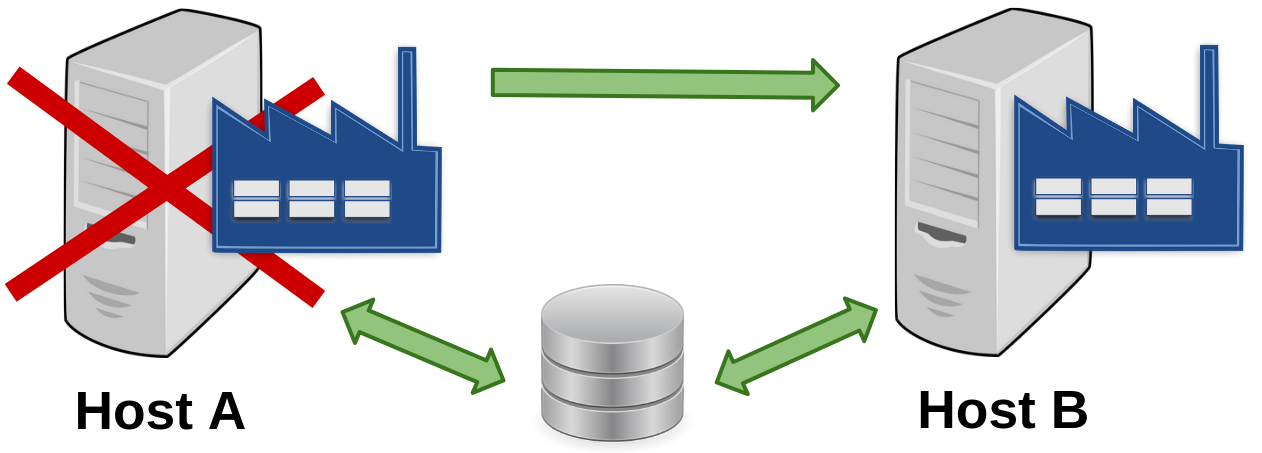
\includegraphics[width=6cm,clip]{images/K8SResilience}
\caption{When a physical host goes down in Kubernetes, the factory pod will automatically restart on another host in the cluster}
\label{K8SResilience}
\end{figure}

By migrating to K8s, the OSG Factory achieves a more resilient and automated deployment model, significantly improving reliability compared to traditional bare metal infrastructure.

\section{Conclusions}
\label{conclusions}

Migrating the OSG Factory to K8s has significantly improved its resilience, maintainability, and automation compared to traditional bare metal deployments. By leveraging containerization, GitOps workflows, and K8s' built-in fault tolerance, we have created a modern, scalable infrastructure that reduces operational overhead and minimizes downtime. The factory now benefits from automatic recovery in the event of node failures, persistent storage for critical state data, and a fully automated deployment process that integrates seamlessly with the broader infrastructure of the OSG.

While this migration represents a major step forward, further improvements are planned. One key area of focus is enhancing tarball management. Currently, operators must manually track and deploy new HTCondor tarballs when they are released. The aim is to improve this process by automating the detection and deployment of new tarballs, ensuring that the factory always runs the latest available software without manual intervention. Additionally, to further enhance redundancy and fault tolerance, we plan to deploy a second factory on the OSG Tempest K8s cluster. This will provide an alternative submission point, reducing the risk of service disruption and increasing overall reliability for both CMS and other VOs that rely on the OSG Factory.

By continuing to refine automation and expand our deployment infrastructure, we aim to further improve the efficiency, reliability, and maintainability of the OSG Factory, ensuring it remains a robust and scalable solution for distributed high-throughput computing.

\section{Acknowledgements}
\label{acknowledgements}
This work was partially supported by the US National Science Foundation under Grant No. 2121686 and under Grant No. 2030508.

\begin{thebibliography}{}
\bibitem{gwms} The Glidein-based Workflow Management System, \url{https://glideinwms.fnal.gov/doc.prd/index.html}

\bibitem{cms} CMS Collaboration, The CMS experiment at the CERN LHC, 
JINST 3 (2008) S08004, doi:10.1088/1748-0221/3/08/S08004.

\bibitem{htcondor} D. Thain, T. Tannenbaum, \& M. Livny, Distributed computing in practice: the Condor experience. {\em Concurrency - Practice And Experience}. \textbf{17}, 323-356 (2005),  doi:10.1002/cpe.938

%\bibitem{htcondor} The HTCondor Software Suite public web site, \url{https://research.cs.wisc.edu/htcondor/index.html}

\bibitem{wlcg} The Worldwide LHC Computing Grid \url{http://wlcg.web.cern.ch}.

\bibitem{globalpool} J. Balcas et al. ``Using the glideinWMS System as a Common Resource Provisioning Layer in CMS'', J. Phys.: Conf. Ser. \textbf{664} 062031 (2015).

\bibitem{osgprojects} OSG Projects that uses GlideinWMS \url{https://osg-htc.org/projects}

\bibitem{docker} The Docker platform \url{https://www.docker.com/}

\bibitem{k8s} The Kubernetes orchestration system \url{https://kubernetes.io/}

\bibitem{OSGfabric} Managing the OSG Fabric
of Services the GitOps Way \url{https://indico.jlab.org/event/459/contributions/11487/attachments/9327/13527/GitOps%20-%20CHEP.pdf}

\end{thebibliography}

\end{document}

% end of file template.tex

<div id='footer'><table width='100%'><tr><td class='right'><a href='http://fusioninventory.org/'><span class='copyright'>FusionInventory 9.1+1.0 | copyleft <img src='/glpi/plugins/fusioninventory/pics/copyleft.png'/>  2010-2016 by FusionInventory Team</span></a></td></tr></table></div>